%! Author = matteomagnini
%! Date = 05/03/25

%----------------------------------------------------------------------------------------
\chapter{SKI: methods and contributions}
\label{ch:ski-methods-and-contributions}
\minitoc
%----------------------------------------------------------------------------------------

In this chapter we present two main algorithmic contributions to the field of \gls{SKI}.
%
First, we provide the motivations behind the design and development of these contributions in \Cref{sec:ski-motivations}.
%
Second, we detail the contributions themselves in \Cref{sec:ski-contribution-kill,sec:ski-contribution-kins}, and we report the results of the empirical evaluation of these contributions.
%
Finally, we discuss the implications of these contributions and outline future directions in \Cref{sec:ski-discussion-and-future-direction}.


\section{Motivations}\label{sec:ski-motivations}
%
Aware by the limitations reported in \Cref{subsec:limitations-and-challenges-of-ski}, we wanted to develop novel \gls{SKI} methods that could be used in many different domains.
%
For this reason, these methods include all the elements described in \Cref{subsec:how-to-inject}.
%
In particular, a \emph{parser} is provided to convert symbolic knowledge into a format that can be injected into a neural network.
%
In this way, we are not bounded to a specific knowledge base nor to a specific domain.
%
The transformation of the parsed rules into a numeric interpretation is automatically performed by a \emph{fuzzification step}.
%
Finally, the sub-symbolic component is injected into a neural network, which is trained to learn the symbolic knowledge.
%
Another limitation that we wanted to address is the expressiveness of the symbolic knowledge that can be injected.
%
What we target in these two works is knowledge expressed in \emph{stratified Datalog with negation}.


\subsection{Stratified Datalog with negation}\label{subsec:skistratified-datalog-with-negation}
%
This logic is a variant of Datalog~\cite{DBLP:books/mc/18/MaierTKW18} with no recursion -- neither direct nor indirect -- yet supporting negated atoms.
%
We choose Datalog because of its expressiveness (strictly higher than propositional logic) and its acceptable limitations.
%
The lack of recursion, in particular, prevents issues when it comes to convert formulas into neural structures (which are \glspl{DAG}).
%
Since we rely on Datalog with negation, we allow atoms in the bodies od clauses to be negated.
%
Using the same notation as in \Cref{subsec:datalog}, in case the $i^{th}$ atom in the body of some clause is negated, we write $\neg b_{i}$.
%
There, each atom $h$, $b_{1}$, $b_{2}$, \dots{} may be a predicate of arbitrary arity.

An \(l\)-ary predicate \(p\) denotes a relation among \(l\) entities: \(p(t_1, \dots, t_l)\), where each \(t_i\) is a term, i.e., either a constant (denoted in \texttt{monospace}) representing a particular entity, or a logic variable (denoted by \textit{Capitalised Italic}) representing some unknown entity or value.
%
Well-known binary predicates – e.g., \(>\), \(<\), \(=\) – are admissible, too, and retain their usual semantics from arithmetic.
%
For the sake of readability, we may write these predicates in infix form—hence \(>(X, 1) \equiv X > 1\).

To support injection into a particular \gls{NN}, we further assume the input knowledge base defines one (and only one) outer relation -- say \texttt{output} or \texttt{class} -- involving as many variables as the input and output features the \gls{NN} has been trained upon.
%
That relation must be defined via one clause per output neuron.
%
Yet, each clause may contain other predicates in their bodies, in turn defined by one or more clauses.
%
In that case, since we rely on stratified Datalog, we require the input knowledge to not include any (directly or indirectly) recursive clause definition.

For example, for a 3-class classification task, any provided knowledge base should include a clause such as the following one:
%
\begin{align*}
    \texttt{class}(\bar{X}, y_1) &\leftarrow \texttt{p}_1(\bar{X}) \land \texttt{p}_2(\bar{X}) \\
    \texttt{p}_1(\bar{X}) &\leftarrow \dots \\
    \texttt{p}_2(\bar{X}) &\leftarrow \dots \\
    \texttt{class}(\bar{X}, y_2) &\leftarrow \texttt{p}'_1(\bar{X}) \land \texttt{p}'_2(\bar{X}) \\
    \texttt{p}'_1(\bar{X}) &\leftarrow \dots \\
    \texttt{p}'_2(\bar{X}) &\leftarrow \dots \\
    \texttt{class}(\bar{X}, y_3) &\leftarrow \texttt{p}''_1(\bar{X}) \land \texttt{p}''_2(\bar{X}) \\
    \texttt{p}''_1(\bar{X}) &\leftarrow \dots \\
    \texttt{p}''_2(\bar{X}) &\leftarrow \dots
\end{align*}
%
where \(\bar{X}\) is a tuple having as many variables as the neurons in the output layer, \(y_i\) is a constant denoting the \(i\)-th class, and \(\texttt{p}_1\), \(\texttt{p}_2\), \(\texttt{p}'_1\), \(\texttt{p}'_2\), \(\texttt{p}''_1\), \(\texttt{p}''_2\) are ancillary predicates defined via Horn clauses as well.


\section{Knowledge injection via lambda layer}\label{sec:ski-contribution-kill}
%
In this section we present the paper ``A view to a KILL: Knowledge Injection via Lambda Layer''~\cite{DBLP:conf/woa/MagniniCO22}, presented at the 23rd Workshop ``From Objects to Agents'' (WOA 2022)~\footnote{\url{https://sites.google.com/view/woa2022/}}.
%
The paper introduces a novel \gls{SKI} method, called \gls{KILL}, which allow to inject symbolic knowledge in stratified Datalog with negation into \glspl{NN} of any shape.
%
\Gls{KILL} does not require the input formulas to be \emph{ground}, and it does not impose any constraint on the \gls{NN} undergoing injection.
%
The method acts directly at the backpropagation level, by increasing the penalty to be back-propagated whenever the \gls{NN} output is violating the knowledge to be injected.
%
For this reason, \gls{KILL} falls under the \emph{guided learning} strategy, as described in \Cref{subsec:how-to-inject}.


\subsection{$\Lambda$-layer}\label{subsec:lambda-layer}
%
\begin{figure}
    \centering
    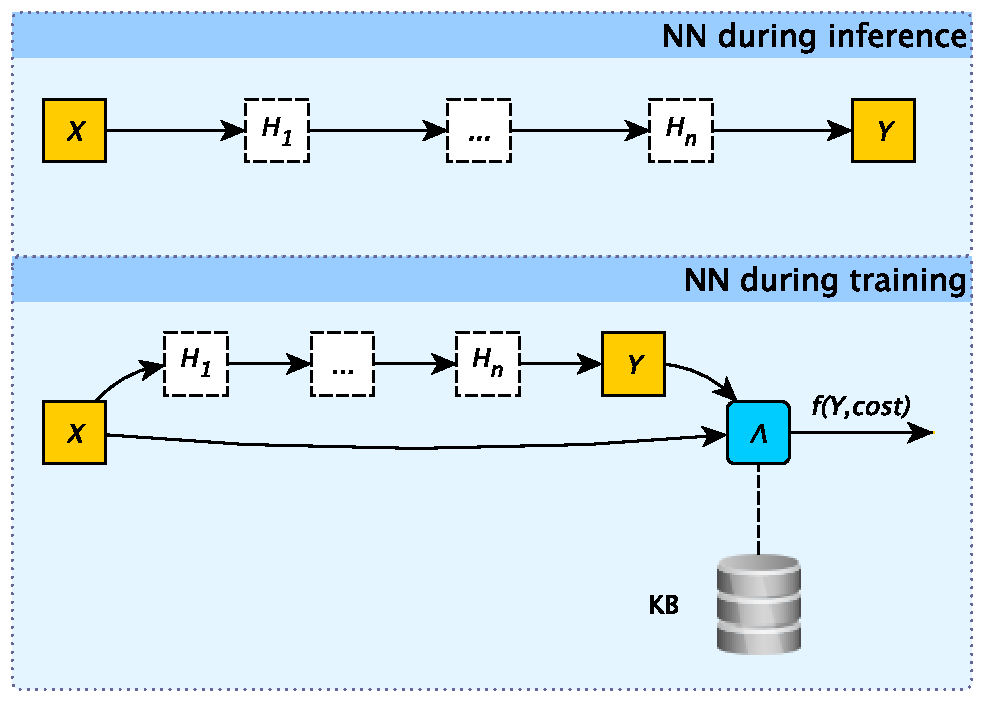
\includegraphics[width=0.8\linewidth]{figures/lambda-layer}
    \caption[General architecture of a NN with $\Lambda$-layer]{
        General architecture of a \gls{NN} with $n$ hidden layers, $X$ and $Y$ are respectively the input and output layers.
        %
        Before training, \gls{KILL} is applied to the predictor so that a new model constrained by the knowledge base (KB) is obtained.
        %
        The $\Lambda$-layer is added to the output layer, and then removed for the inference phase.
    }
    \label{fig:lambda-layer}
\end{figure}
%
The idea behind \gls{KILL} is to perform injection during training.
%
The injection is performed by appending one further layer -- the \emph{$\Lambda$-layer} -- at the output end of the \gls{NN}, and by training the overall network as usual (e.g., via gradient descent or similar).
%
The $\Lambda$-layer introduces an error whenever the prediction from the network's output layer violates the symbolic knowledge being injected.
%
This error influences the gradient descent or other optimization functions, discouraging violations of the symbolic knowledge.
%
In essence, the \gls{NN} learns inductively to avoid wrong predictions by penalizing violations during training.
%
To achieve this, the $\Lambda$-layer employs a custom activation function that modifies the output of the network's original output layer.
%
Additionally, the symbolic knowledge must be numerically interpreted, converting logical formulas into real-valued functions to compute error values.
%
Once the training phase is complete, the $\Lambda$-layer can be removed, leaving the original network architecture intact.


To elaborate on the $\Lambda$-layer, we consider a symbolic knowledge base, denoted as \(\mathcal{K}\), to be injected into a feedforward \gls{NN} of arbitrary depth, denoted as \(\mathcal{N}\).
%
Let \(\mathcal{N}\) have an input layer \(\mathbf{X}\) and an output layer \(\mathbf{Y}\), where \(\mathbf{Y}\) is assumed to be of shape \(n \times 1\).
%
This discussion applies to layers of any shape, including multidimensional ones.
%
No assumptions are made about the activation function of \(\mathbf{Y}\), the topology or nature of the hidden layers, or the shape of \(\mathbf{X}\).
%
The output of \(\mathbf{Y}\) is denoted as \(\mathbf{y} = [y_1, \dots, y_n]\), representing the network's prediction for a given input \(\mathbf{x}\).
%
The knowledge base \(\mathcal{K}\) consists of \(n\) rules, \(\mathcal{K} = \{\varphi_1, \dots, \varphi_n\}\), where each rule \(\varphi_i\) constrains the relationship between \(\mathbf{x}\) and \(y_i\).


To inject \(\mathcal{K}\), the $\Lambda$-layer is added to the network architecture, as illustrated in \Cref{fig:lambda-layer}.
%
This layer is densely connected to both \(\mathbf{X}\) and \(\mathbf{Y}\), and its activation function introduces a penalty on \(y_i\) whenever the corresponding rule \(\varphi_i\) is violated for an input-output pair \((\mathbf{x}, \mathbf{y})\).
%
The output of the $\Lambda$-layer, denoted as \(\boldsymbol{\lambda}\), is defined as:
%
\[
\boldsymbol{\lambda} = \mathbf{y} \times (1 + \mathbf{C}(\mathbf{x}, \mathbf{y}))
\]
%
where \(\mathbf{C}(\mathbf{x}, \mathbf{y})\) is a positive penalty vector representing the cost of modifying the network's output \(\mathbf{y}\).
%
The penalty vector \(\mathbf{C}(\mathbf{x}, \mathbf{y})\) is given by:
%
\[
\mathbf{C}(\mathbf{x}, \mathbf{y}) = [c_1(\mathbf{x}, y_1), \dots, c_i(\mathbf{x}, y_i), \dots, c_n(\mathbf{x}, y_n)]
\]
%
where \(c_i : \mathbf{X} \times \mathbf{Y} \to [0, 1]\) interprets the rule \(\varphi_i\) as a cost in the range \([0, 1]\) for the given values of \(\mathbf{x}\) and \(y_i\).
%
A penalty is applied to the \(i\)-th neuron of \(\mathbf{Y}\) whenever the corresponding rule \(\varphi_i\) is violated.
%
The penalty is higher when the violation is severe and approaches zero when the violation is minimal or absent.


\subsection{KILL fuzzifier}\label{subsec:kill-fuzzifier}
%
% !TeX spellcheck = en_GB
% !TeX root = ../phd-thesis.tex

\begin{table}
    \centering
    %
    \begin{tabular}{l|r||cl|r}
        \textbf{Formula} & \textbf{C. interpretation} & & \textbf{Formula} & \textbf{C. interpretation}
        \\
        \hline\hline
        $\llbracket\neg \phi\rrbracket$ & $\eta(1 - \llbracket\phi\rrbracket)$ & & $\llbracket\phi \le \psi\rrbracket$  & $\eta(\llbracket\phi\rrbracket - \llbracket\psi\rrbracket)$
        \\
        $\llbracket\phi  \wedge \psi\rrbracket$ &  $\eta(max(\llbracket\phi\rrbracket, \llbracket\psi\rrbracket))$ & & $\llbracket \pred{class}(\bar{X}, \const{y}_i) \leftarrow \psi \rrbracket$ & $\llbracket \psi \rrbracket^{*}$
        \\
        $\llbracket\phi  \vee \psi\rrbracket$ & $\eta(min(\llbracket\phi\rrbracket, \llbracket\psi\rrbracket))$ & & $\llbracket \text{expr}(\bar{X}) \rrbracket$ & $\text{expr}(\llbracket\bar{X}\rrbracket)$
        \\
        $\llbracket\phi = \psi\rrbracket$ & $\eta(|\llbracket\phi\rrbracket-\llbracket\psi\rrbracket|)$ & & $\llbracket \mathtt{true} \rrbracket$ & $0$
        \\
        $\llbracket\phi \ne \psi\rrbracket$ & $\llbracket \neg ( \phi = \psi )\rrbracket$ & & $\llbracket \mathtt{false} \rrbracket$ & $1$
        \\
        $\llbracket\phi > \psi\rrbracket$  & $\eta(0.5 - \llbracket\phi\rrbracket + \llbracket\psi\rrbracket) $ & & $\llbracket X \rrbracket$ & $x$
        \\
        $\llbracket\phi \ge \psi\rrbracket$ & $\eta(\llbracket\psi\rrbracket - \llbracket\phi\rrbracket)$ & & $\llbracket \const{k} \rrbracket$ & $k$
        \\
        $\llbracket\phi < \psi\rrbracket$  &  $\eta(0.5 + \llbracket\phi\rrbracket - \llbracket\psi\rrbracket)$ & & $\llbracket \pred{p}(\bar{X}) \rrbracket^{**}$ & $\llbracket \psi_1 \vee \ldots \vee \psi_k \rrbracket$
        
    \end{tabular}
    %
    \begin{center}\scriptsize
        $^{*}$ encodes the penalty for the $i^{th}$ neuron
        \\
        \smallskip
        $^{**}$ assuming predicate $p$ is defined by $k$ clauses of the form:
        \\
        $\pred{p}(\bar{X}) \leftarrow \psi_1,\ \ldots,\ \pred{p}(\bar{X}) \leftarrow \psi_k$
    \end{center}
    %
    \caption[KILL Fuzzifier: Logic Formulae Encoding]{
        Logic formulas' encoding into real-valued functions.
        %
        There, $X$ is a logic variable, while $x$ is the corresponding real-valued variable, whereas is $\bar{X}$ a tuple of logic variables.
        %
        Similarly, $\const{k}$ is a numeric constant, and $k$ is the corresponding real value, whereas $\const{k}_i$ is the constant denoting the $i^{th}$ class of a classification problem.
        %
        Finally, $\text{expr}(\bar{X})$ is an arithmetic expression involving the variables in $\bar{X}$.
    }
    %
    \label{tab:kill-logic-formulae}
    %
\end{table}
%
% !TeX spellcheck = en_GB
% !TeX root = ../phd-thesis.tex

\begin{figure*}[t]
    \centering
    \def\astscale{0.4}
    \begin{minipage}[c]{0.4\textwidth}
        \centering
        \begin{subfigure}{\linewidth}
            \centering
            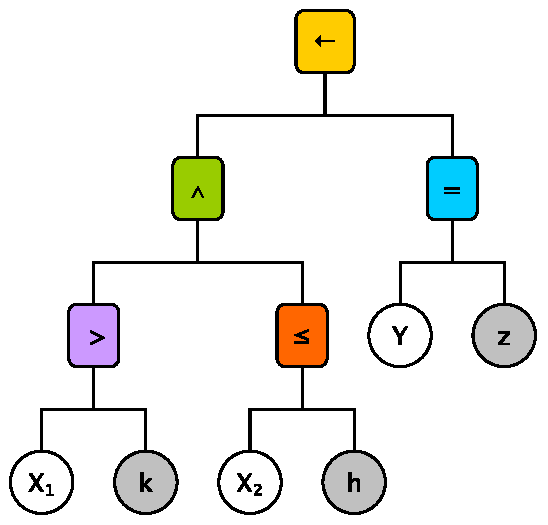
\includegraphics[scale=\astscale]{figures/ast-unencoded}
            \subcaption{AST of a logic formula}
            \label{fig:ast-kill-unencoded}
        \end{subfigure}
        \vspace{1.5ex}
        \tikz{\draw[->, thick] (0,0) -- (0,-0.4);}
        \vspace{2ex}
        \begin{subfigure}{\linewidth}
            \centering
            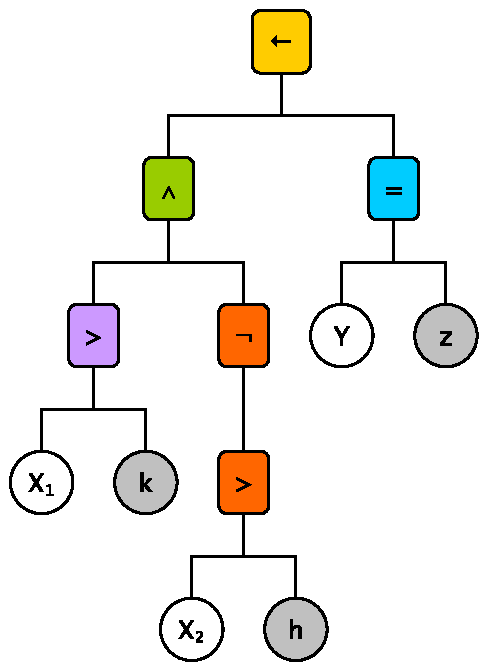
\includegraphics[scale=\astscale]{figures/ast-simplified}
            \subcaption{Simplified AST of a logic formula}
            \label{fig:ast-kill-simplified}
        \end{subfigure}
    \end{minipage}
    \hspace{0.5cm}
    \raisebox{-1cm}{\tikz{\draw[->, thick] (0,0) -- (0.7,0);}}
    \hspace{0.5cm}
    \begin{minipage}[c]{0.4\textwidth}
        \centering
        \begin{subfigure}{\linewidth}
            \centering
            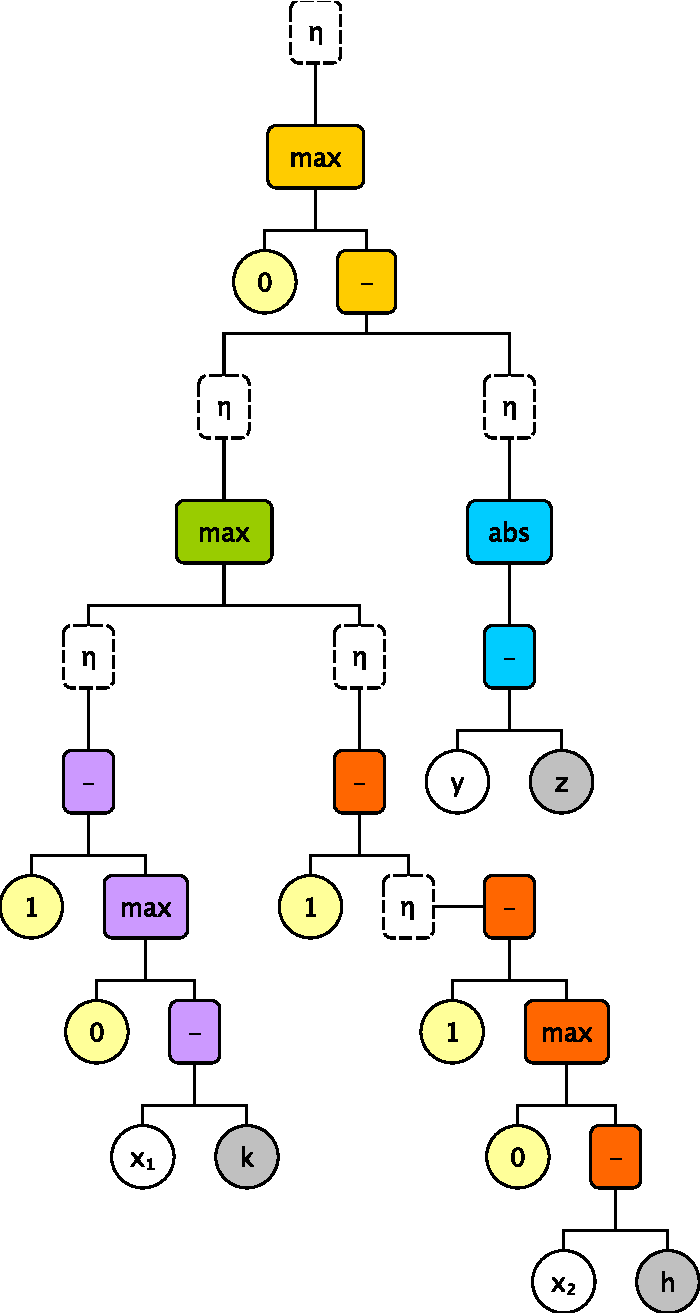
\includegraphics[scale=\astscale]{figures/ast-encoded}
            \subcaption{AST of the same formula, encoded as real-valued function}
            \label{fig:ast-kill-encoded}
        \end{subfigure}
    \end{minipage}
    \caption[KILL Encoding of logic formulas into real-valued functions]{
        %
        Example of the encoding process of logic formulas into real-valued functions.
        %
        Only \gls{AST} are depicted.
        %
        Boxes coloured in the same way represent the encoding of a given operator through each encoding step.
        %
        For instance, operator $<$ (red) is first converted into a negated $\geq$, and then into a combination of $max$ and subtractions.
    }
    \label{fig:ast-kill}
\end{figure*}

%
Before injecting symbolic knowledge into a neural network, each formula associated with an output neuron must be converted into a real-valued function to compute the cost of violating that formula.

This conversion relies on a multivalued interpretation of logic inspired by \L{}ukasiewicz's logic~\cite{DBLP:journals/jsyml/Hay63}.
%
Each formula is encoded using the \(\llbracket \cdot \rrbracket\) function, which maps logical formulas to real-valued functions.
%
These functions accept real vectors of size \(m + n\) as input and return scalars in \(\mathbb{R}\) as output.
%
The resulting scalars are clipped to the \([0, 1]\) range using the \(\eta : \mathbb{R} \to [0, 1]\) function, defined as:
%
\begin{equation}
    \label{eq:eta-function}
    \eta(x) =
    \begin{cases}
        0 & \text{if } x \leq 0, \\
        x & \text{if } 0 < x < 1, \\
        1 & \text{if } x \geq 1.
    \end{cases}
\end{equation}

The values obtained from \(\eta(x)\) represent penalties, as discussed in \Cref{subsec:lambda-layer}.
%
The penalty for the \(i^{\text{th}}\) neuron violating rule \(\varphi_i\) is expressed as \(c_i(\mathbf{x}, y_i) = \eta(\llbracket \varphi_i \rrbracket(\mathbf{x}, y_i))\).

The \(\llbracket \cdot \rrbracket\) encoding function is recursively defined in \Cref{tab:kill-logic-formulae}.
%
To compute the penalty \(c_i(\mathbf{x}, y_i)\) for the \(i^{\text{th}}\) neuron, \gls{KILL} identifies the Datalog rule of the form:
%
\begin{align*}
    \texttt{class}(\bar{X}, y_i) &\leftarrow \psi.
\end{align*}
%
The method focuses on the body \(\psi\) of the rule, ignoring its head, as the head specifies the expected output for the rule.
%
If \(\psi\) contains predicates \(p_1, p_2\), defined by one or more clauses in the knowledge base, these predicates are replaced by the disjunction of the bodies of all clauses defining them.
%
This process is repeated until \(\psi\) contains only binary expressions involving input variables, constants, arithmetic operators, and logical connectives.
%
Finally, operators and connectives are replaced by continuous functions, as detailed in \Cref{tab:kill-logic-formulae}.
%
The entire process produces a real-valued interpretation of the original formula, which \gls{KILL} uses to compute \(c_i(\mathbf{x}, y_i)\).

\Cref{fig:ast-kill} illustrates an example of the encoding process.
%
The example formula is:
%
\begin{align*}
    \texttt{class}(X_1, X_2, z) &\leftarrow (X_1 \geq k) \land (X_2 \geq h),
\end{align*}
%
where \(k\), \(h\), and \(z\) are numeric constants, \(X_1\) and \(X_2\) are input variables, and \(Y\) is an output variable.
%
\Cref{fig:ast-kill-unencoded} shows the \gls{AST} of this formula.
%
\Cref{fig:ast-kill-simplified} depicts the same \gls{AST} after replacing the \(\leq\) operator with a negated \(>\) operator.
%
Finally, \Cref{fig:ast-kill-encoded} shows the \gls{AST} of the encoded function.
%
A public implementation of \gls{KILL} available on \gls{PSyKI}~\cite{DBLP:conf/atal/MagniniCO22}\footnote{\label{foot:psyki}\url{https://github.com/psykei/psyki-python}}.


\subsection{Validation}\label{subsec:kill-validation}
%
% !TeX spellcheck = en_GB
% !TeX root = ../phd-thesis.tex

\begin{table}[!t]
    \centering
    % \begin{adjustbox}{width=0.8\linewidth,center}
    \begin{tabular}{l|r|r|r|r}
        \textbf{Class} & \makecell{\textbf{Train.}\\\textbf{Instances}} & \makecell{\textbf{Train.}\\\textbf{Freq. (\%)}} & \makecell{\textbf{Test}\\\textbf{Instances}} & \makecell{\textbf{Test}\\\textbf{Freq. (\%)}}
        \\\hline\hline
        \text{high card} & 12,493 &  49.95 & 501,209 &  50.12
        \\
        \text{pair} & 10,599 & 42.38 & 422,498 & 42.25
        \\
        \text{two pairs} & 1,206 & 4.82 & 47,622 & 4.76
        \\
        \text{three of a kind} & 513 & 2.05 & 21,121 & 2.11
        \\
        \text{straight} & 93 & 0.37 & 3,885 & 0.39
        \\
        \text{flush} & 54 & 0.22 & 1,996 & 0.2
        \\
        \text{full house} & 36 & 0.14 & 1,424 & 0.14
        \\
        \text{four of a kind} & 6 & 0.024 & 230 & 0.023
        \\
        \text{straight flush} & 5 & 0.02 & 12 & 0.001
        \\
        \text{royal flush} & 5 &  0.02 & 3 & \scinum{3}{-4}
        \\
        \hline
        \textbf{Total} & 25,010 & 100 & 1,000,000 & 100
    \end{tabular}
    % \end{adjustbox}
    \caption[PHDS statistics per class]{
        \Gls{PHDS} statistics per class.
        %
        The dataset is heavily imbalanced, with the \emph{high card} class being the most frequent.
        %
        Considering together the two most frequent classes, \emph{high card} and \emph{pair}, they account for over 92\% of the training instances.
    }
    \label{tab:phds-dataset}
\end{table}
%
The method has been validated on the \glsentrylong{PHDS} (\glsentryshort{PHDS})~\cite{poker_hand_158}, a dataset for poker hand classification.
%
The task consists in a multiclass classification problem on a finite -- yet very large -- discrete domain.
%
Classes are overlapped and heavily imbalanced, but exact classification rules can be written in logic formulas.
%
\Gls{PHDS} has $1,025,010$ records\footnote{the size of the input space is the amount 5-permutations of 52 cards, i.e., $\frac{52!}{(52 - 5)!}$}, each with $10$ features, and $1$ output class.
%
Each record represents a poker hand of $5$ cards, each card is identified by two features: a rank and a suit.
%
Suit is a categorical feature (e.g., \texttt{spades}, \texttt{hearts}, \texttt{diamonds}, \texttt{clubs}), while rank is a numeric feature (e.g., $1$ for Ace, $2$ for Two, \dots, $13$ for King).
%
Each hand can be classified as one of $10$ different classes denoting the poker hand type (e.g., \texttt{high card}, \texttt{pair}, \texttt{two pairs}, \texttt{three of a kind}, etc.).
%
\Cref{tab:phds-dataset} reports the statistics of the dataset per class for both training and test sets.


\paragraph{\Gls{PHDS} logic rules}\label{par:phds-logic-rules}
%
% !TeX spellcheck = en_GB
% !TeX root = ../phd-thesis.tex

\begin{table}
    \centering
    \begin{adjustbox}{width=\linewidth, center}
        \begin{tabular}{c|p{1.385\linewidth}}
            \textbf{Class} & \textbf{Logic Formulation}
            \\\hline\hline
            Pair & $\begin{array}{l}
                \pred{class}(R_1, \ldots, S_5, \const{pair}) \leftarrow \pred{pair}(R_1, \ldots, S_5)
                \\
                \pred{pair}(R_1, \ldots, S_5) \leftarrow R_1 = R_2
                \\
                \pred{pair}(R_1, \ldots, S_5) \leftarrow R_1 = R_3
                \\
                \pred{pair}(R_1, \ldots, S_5) \leftarrow R_1 = R_4
                \\
                \pred{pair}(R_1, \ldots, S_5) \leftarrow R_1 = R_5
                \\
                \pred{pair}(R_1, \ldots, S_5) \leftarrow R_2 = R_3
                \\
                \pred{pair}(R_1, \ldots, S_5) \leftarrow R_2 = R_4
                \\
                \pred{pair}(R_1, \ldots, S_5) \leftarrow R_2 = R_5
                \\
                \pred{pair}(R_1, \ldots, S_5) \leftarrow R_3 = R_4
                \\
                \pred{pair}(R_1, \ldots, S_5) \leftarrow R_3 = R_5
                \\
                \pred{pair}(R_1, \ldots, S_5) \leftarrow R_4 = R_5
            \end{array}$
            \\\hdashline
            Two Pairs & $\begin{array}{l}
                \pred{class}(R_1, \ldots, S_5, \const{two}) \leftarrow \pred{two}(R_1, \ldots, S_5)
                \\
                \pred{two}(R_1, \ldots, S_5) \leftarrow R_1 = R_2 \wedge R_3 = R_4
                \\
                \pred{two}(R_1, \ldots, S_5) \leftarrow R_1 = R_3 \wedge R_2 = R_4
                \\
                \pred{two}(R_1, \ldots, S_5) \leftarrow R_1 = R_4 \wedge R_2 = R_3
                \\
                \pred{two}(R_1, \ldots, S_5) \leftarrow R_1 = R_2 \wedge R_3 = R_5
                \\
                \pred{two}(R_1, \ldots, S_5) \leftarrow R_1 = R_3 \wedge R_3 = R_5
                \\
                \pred{two}(R_1, \ldots, S_5) \leftarrow R_1 = R_5 \wedge R_2 = R_3
                \\
                \pred{two}(R_1, \ldots, S_5) \leftarrow R_1 = R_2 \wedge R_4 = R_5
                \\
                \pred{two}(R_1, \ldots, S_5) \leftarrow R_1 = R_4 \wedge R_2 = R_5
                \\
                \pred{two}(R_1, \ldots, S_5) \leftarrow R_1 = R_5 \wedge R_2 = R_4
                \\
                \pred{two}(R_1, \ldots, S_5) \leftarrow R_1 = R_3 \wedge R_4 = R_5
                \\
                \pred{two}(R_1, \ldots, S_5) \leftarrow R_1 = R_4 \wedge R_3 = R_5
                \\
                \pred{two}(R_1, \ldots, S_5) \leftarrow R_1 = R_5 \wedge R_3 = R_4
                \\
                \pred{two}(R_1, \ldots, S_5) \leftarrow R_2 = R_3 \wedge R_4 = R_5
                \\
                \pred{two}(R_1, \ldots, S_5) \leftarrow R_2 = R_4 \wedge R_3 = R_5
                \\
                \pred{two}(R_1, \ldots, S_5) \leftarrow R_2 = R_5 \wedge R_3 = R_4
            \end{array}$
            \\\hdashline
            Three of a Kind & $\begin{array}{l}
                \pred{class}(R_1, \ldots, S_5, \const{three}) \leftarrow \pred{three}(R_1, \ldots, S_5)
                \\
                \pred{three}(R_1, \ldots, S_5) \leftarrow R_1 = R_2 \wedge R_1 = R_3
                \\
                \pred{three}(R_1, \ldots, S_5) \leftarrow R_1 = R_2 \wedge R_1 = R_4
                \\
                \pred{three}(R_1, \ldots, S_5) \leftarrow R_1 = R_2 \wedge R_1 = R_5
                \\
                \pred{three}(R_1, \ldots, S_5) \leftarrow R_1 = R_3 \wedge R_1 = R_4
                \\
                \pred{three}(R_1, \ldots, S_5) \leftarrow R_1 = R_3 \wedge R_1 = R_5
                \\
                \pred{three}(R_1, \ldots, S_5) \leftarrow R_1 = R_4 \wedge R_1 = R_5
                \\
                \pred{three}(R_1, \ldots, S_5) \leftarrow R_2 = R_3 \wedge R_2 = R_4
                \\
                \pred{three}(R_1, \ldots, S_5) \leftarrow R_2 = R_3 \wedge R_2 = R_5
                \\
                \pred{three}(R_1, \ldots, S_5) \leftarrow R_2 = R_4 \wedge R_2 = R_5
                \\
                \pred{three}(R_1, \ldots, S_5) \leftarrow R_3 = R_4 \wedge R_3 = R_5
            \end{array}$
            \\\hdashline
            Straight & $\begin{array}{l}
                \pred{class}(R_1, \ldots, S_5, \const{straight}) \leftarrow \pred{royal}(R_1, \ldots, S_5)
                \\
                \pred{class}(R_1, \ldots, S_5, \const{straight}) \leftarrow \pred{straight}(R_1, \ldots, S_5)
                \\
                \pred{straight}(R_1, \ldots, S_5) \leftarrow (R_1 + R_2 + R_3 + R_4 + R_5) = (5 * \text{min}(R_1, \ldots, R_5) + 10) \wedge \neg \pred{pair}(R_1, \ldots, S_5)
                \\
                \pred{royal}(R_1, \ldots, S_5) \leftarrow \text{min}(R_1, \ldots, R_5) = 1 \wedge (R_1 + R_2 + R_3 + R_4 + R_5 = 47) \wedge \neg \pred{pair}(R_1, \ldots, S_5)
                \\
            \end{array}$
            \\\hdashline
            Flush & $\begin{array}{l}
                \pred{class}(R_1, \ldots, S_5, \const{flush}) \leftarrow \pred{flush}(R_1, \ldots, S_5)
                \\
                \pred{flush}(R_1, \ldots, S_5) \leftarrow S_1 = S_2 \wedge S_1 = S_3 \wedge S_1 = S_4 \wedge S_1 = S_5
            \end{array}$
            \\\hdashline
            Four of a Kind & $\begin{array}{l}
                \pred{class}(R_1, \ldots, S_5, \const{four}) \leftarrow \pred{four}(R_1, \ldots, S_5)
                \\
                \pred{four}(R_1, \ldots, S_5) \leftarrow R_1 = R_2 \wedge R_1 = R_3 \wedge R_1 = R_4
                \\
                \pred{four}(R_1, \ldots, S_5) \leftarrow R_1 = R_2 \wedge R_1 = R_3 \wedge R_1= R_5
                \\
                \pred{four}(R_1, \ldots, S_5) \leftarrow R_1 = R_2 \wedge R_1 = R_4 \wedge R_1 = R_5
                \\
                \pred{four}(R_1, \ldots, S_5) \leftarrow R_1 = R_3 \wedge R_1 = R_4 \wedge R_1 = R_5
                \\
                \pred{four}(R_1, \ldots, S_5) \leftarrow R_2 = R_3 \wedge R_2 = R_4 \wedge R_2 = R_5
            \end{array}$
            \\\hdashline
            Full House & $\begin{array}{l}
                \pred{class}(R_1, \ldots, S_5, \const{full}) \leftarrow three(S_1,\dots,R_5) \wedge two(S_1,\dots,R_5) \wedge \neg four(S_1,\dots,R_5)
            \end{array}$
            \\\hdashline
            Straight Flush & $\begin{array}{l}
                \pred{class}(R_1, \ldots, S_5, \const{straight\_flush}) \leftarrow \pred{straight}(R_1, \ldots, S_5) \wedge \pred{flush}(R_1, \ldots, S_5)
                \\
                 \pred{class}(R_1, \ldots, S_5, \const{straight\_flush}) \leftarrow \pred{royal}(R_1, \ldots, S_5) \wedge \pred{flush}(R_1, \ldots, S_5)
            \end{array}$
            \\\hdashline
            Royal Flush & $\begin{array}{l}
                \pred{class}(R_1, \ldots, S_5, \const{royal}) \leftarrow \pred{royal}(R_1, \ldots, S_5) \wedge \pred{flush}(R_1, \ldots, S_5)
            \end{array}$
            \\\hdashline
            High Card & $\begin{array}{l}
                \pred{class}(R_1, \ldots, S_5, \const{nothing}) \leftarrow \neg \pred{pair}(R_1, \ldots, S_5) \wedge \neg \pred{flush}(R_1, \ldots, S_5) \wedge \neg \pred{straight}(R_1, \ldots, S_5) \wedge \neg \pred{royal}(R_1, \ldots, S_5)
            \end{array}$
        \end{tabular}
    \end{adjustbox}
    \caption{
        Stritified datalog with negation formulas describing poker hands.
        %
        For the sake of readability variables in the head of formulas and in the arguments of predicates are abbreviated.
    }
    \label{tab:phds-logic-rules}
\end{table}
%
We define a \emph{class} rule for each class, encoding the correct way of classifying a poker hand.
%
For instance, let $\{R_{1}, S_{1}, \dots, R_{5}, S_{5}\}$ be the logic variables representing a poker hand (i.e., $R$ for rank and $S$ for suit), then for class \texttt{flush} we have:
%
\begin{equation}\label{eq:flush-class}
     \begin{array}{rcl}
        \pred{class}(R_1, S_1, \ldots, R_5, S_5, \const{flush}) & \leftarrow & \pred{flush}(R_1, S_1, \ldots, R_5, S_5)
        \\
        \pred{flush}(R_1, S_1, \ldots, R_5, S_5) & \leftarrow & S_1 = S_2 \wedge S_1 = S_3 \wedge S_1 = S_4 \wedge S_1 = S_5
    \end{array}
\end{equation}
%
All other rules have the same structure as \Cref{eq:flush-class}: the left-hand side declares the expected class, while the right-hand side describes the necessary conditions for that class—possibly, via some ancillary predicates such as \emph{flush}.
%
\Cref{tab:phds-logic-rules} provides an overview of all the rules we rely upon in our experiments.


\paragraph{Methodology}\label{par:phds-methodology}
%
We adopt the same data partitioning strategy proposed by the dataset authors~\cite{poker_hand_158}.
%
Specifically, the training set consists of $25,010$ samples, while the test set includes $1,000,000$ samples.
%
This unusual ratio between training and test set sizes makes the task more challenging but ensures more reliable results.

For all experiments, we use a fully connected \gls{NN} with three layers.
%
The first two layers consist of $128$ neurons each, while the output layer has $10$ neurons, corresponding to the number of classes.
%
The activation function for the first two layers is \gls{ReLU}, whereas the output layer uses softmax.
%
The network is trained using categorical cross-entropy as the loss function.

We set the batch size to $32$ and train the network for up to $100$ epochs.
%
To evaluate the network's performance, we rely on metrics such as accuracy, macro-F1, and weighted-F1 scores.
%
After training, the \(\Lambda\)-layer is removed, and the resulting \gls{NN} is used for inference.

To prevent overfitting, we employ three stopping criteria during training.
%
First, for 99\% of the training examples, the activation of every output unit must be within 0.25 of the correct value.
%
Second, training stops after 100 epochs.
%
Third, the predictor must achieve at least 90\% accuracy on the training examples but show no improvement in classification performance for five consecutive epochs.
%
These criteria are inspired by previous work~\cite{Towell90}.
%
Finally, we conduct 30 runs for each configuration to obtain a statistically significant population for comparisons.


\paragraph{Results and discussion}\label{par:phds-results}
%
% !TeX spellcheck = en_GB
% !TeX root = ../phd-thesis.tex

\begin{table}
    \centering
     \begin{adjustbox}{width=\linewidth,center}
         \begin{tabular}{l|rr||l|rr}
             \textbf{Metric} & \textbf{Uneducated} & \textbf{Educated} & \textbf{Metric} & \textbf{Uneducated} & \textbf{Educated}
             \\
             \hline\hline
             \textbf{Accuracy} & 0.962 & 0.978 & \textbf{Acc. Straight} & 0.415 & 0.509
             \\
             \textbf{Macro-F1} & 0.512 & 0.538 & \textbf{Acc. Flush} & 0.002 & 0.002
             \\
             \textbf{Weighted-F1} & 0.96 & 0.977 & \textbf{Acc. Full} & 0.628 & 0.69
             \\
             \textbf{Acc. High Card} & 0.977 & 0.989 & \textbf{Acc. Four} & 0.186 & 0.19
             \\
             \textbf{Acc. Pair} & 0.968 & 0.985 & \textbf{Acc. Straight F.} & 0.003 & 0
             \\
             \textbf{Acc. Two Pairs} & 0.867 & 0.914 & \textbf{Acc. Royal F.} & 0 & 0
             \\
             \textbf{Acc. Three} & 0.913 & 0.922 & & &
        \end{tabular}
     \end{adjustbox}
    \caption{
        Test set accuracy, macro-F1 and weighted-F1 on all classes and single mean class accuracies.
        %
        All measures represent the mean over the experiment population (30).
        %
        The Wilcoxon signed-rank test shows that for the accuracy, macro-F1 and weighted-F1 metrics the educated model is significantly better than the uneducated one ($p < 0.05$).
        %
        Also, the educated model is significantly better than the uneducated one for the single mean class accuracies, except for \emph{high card}, \emph{pair} and \emph{straight} classes.
    }
    \label{tab:phds-kill-results}
\end{table}
%
\begin{figure}
    \centering
    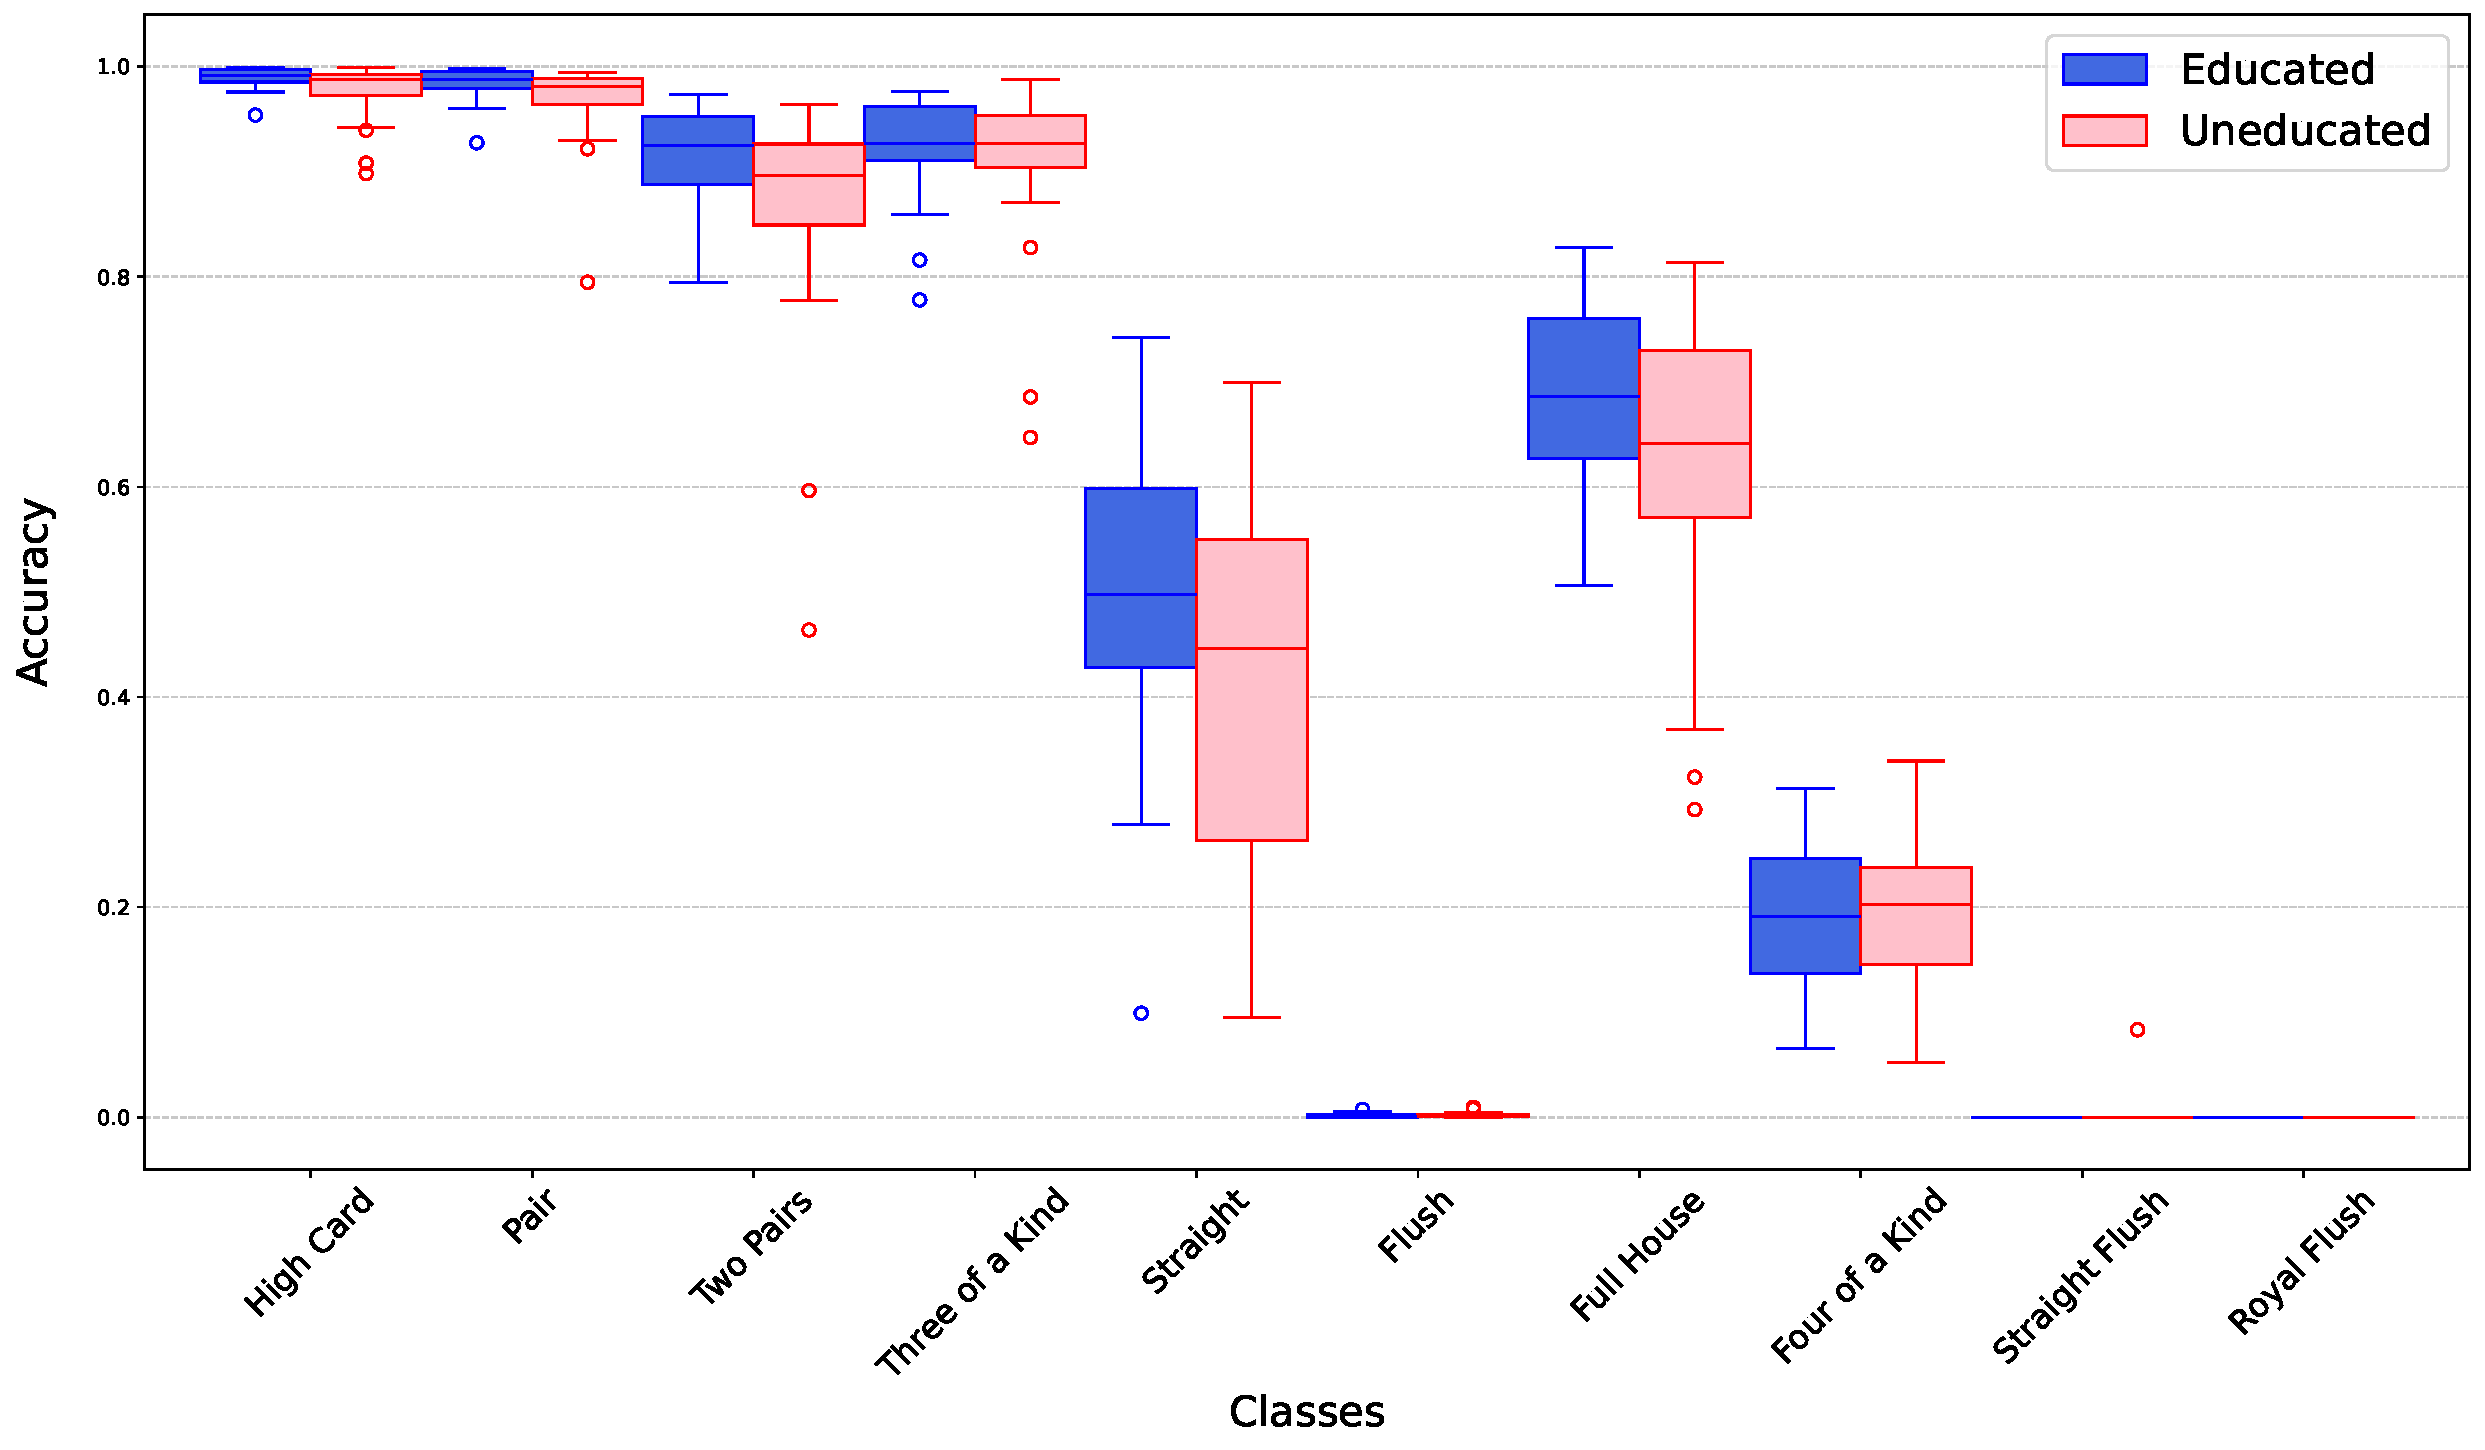
\includegraphics[width=\linewidth]{figures/phds-kill-results}
    \caption[PHDS KILL results]{
        Per class results of the experiments on the \gls{PHDS} dataset using \gls{KILL}.
        %
        The \gls{KILL} method outperforms the uneducated \gls{NN} in the prediction of almost all classes.
        %
        For all class prediction, the Wilcoxon signed-rank test has been applied to compare the two configurations.
        %
        With a p-value threshold of $0.05$, we reject the null hypothesis in the case of \emph{high card}, \emph{pair}, and \emph{straight} classes.
    }
    \label{fig:phds-kill-results}
\end{figure}
%
We define two different configurations for experiments:
%
\begin{inlinelist}
    %
    \item ``uneducated'', where we use the \gls{NN} described in \Cref{par:phds-methodology},
    %
    \item ``educated'', where we apply \gls{KILL} on the same network architecture.
    %
\end{inlinelist}
%
For both configurations we use the same hyperparameters and perform $30$ runs.
%
Results are reported in \Cref{tab:phds-kill-results} and in \Cref{fig:phds-kill-results}.
%
In general, experiments show that both predictors are very good at classifying frequent classes such as \emph{high card} and \emph{pair}.
%
Also for less frequent classes, \emph{two pairs} and \emph{three of a kind}, accuracy is still high.
%
The remaining six classes represent the $0.8\%$ of the training set and therefore much more difficult to correctly predict.
%
For \emph{full house} and \emph{straight}, accuracy has middle values, while for the remaining classes accuracy is pretty close to $0$.
%
All of this is quite expected due to the strong imbalance in the distribution of classes.
%
The only remarkable fact is that accuracy is extremely low for class \emph{flush} even if less frequent classes such as \emph{full house} and \emph{four of a kind} have higher accuracy.
%
We hypothesise that this happens because the vast majority of data consists in classes which depend only on the values of rank and therefore the network tends to consider it much more.
%
Indeed, only \emph{flush}, \emph{straight flush} and \emph{royal flush} (about the $0.26\%$ of the training set) depend on the values of suit.
%
Concerning the comparison between the \emph{uneducated} predictor -- with no additional knowledge -- and the \emph{educated} predictor -- obtained by applying KILL algorithm -- results show that the latter has higher performances with statistic significance.
%
The Wilcoxon signed-rank test~\cite{wilcoxon1945} has been applied to compare the two configurations on all the metrics reported in \Cref{tab:phds-kill-results}.
%
In particular, because of the imbalanced nature of the dataset, the test on macro-F1 and weighted-F1 metrics is more reliable than the test on accuracy.
%
The test shows that the \emph{educated} predictor is significantly better than the \emph{uneducated} one for the overall accuracy, macro-F1 and weighted-F1 metrics (with $p < 0.05$).
%
Also, the \emph{educated} predictor is significantly better than the \emph{uneducated} one for the single mean class accuracies, except for \emph{high card}, \emph{pair} and \emph{straight} classes.


\section{Knowledge injection via network structuring}\label{sec:ski-contribution-kins}
%
In this section we present the paper ``KINS: Knowledge Injection via Network Structuring''~\cite{DBLP:conf/cilc/MagniniCO22}, presented at the 37th Italian Conference on Computational Logic (CILC 2022)~\footnote{\url{http://cilc2022.apice.unibo.it/}}.
%
The paper introduces a novel \gls{SKI} methods, named \gls{KINS}, which similarly to \gls{KILL} allows to inject symbolic knowledge in stratified Datalog with negation into \glspl{NN} of any shape.
%
Differently from \gls{KILL}, \gls{KINS} does not act at the backpropagation level, but it modifies the structure of the \gls{NN} to inject symbolic knowledge.
%
Hence, \gls{KINS} falls under the \emph{structuring} strategy, as described in \Cref{subsec:how-to-inject}.


\subsection{KINS architecture}\label{subsec:kins-architecture}
%
\begin{figure}
    \centering
    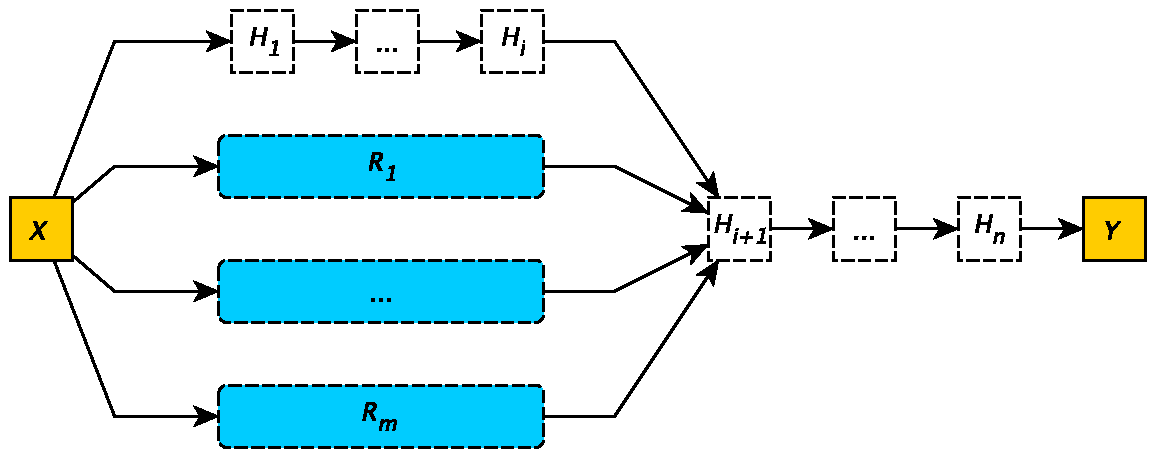
\includegraphics[width=\textwidth]{figures/kins-network-architecture}
    \caption[General architecture of a NN with KINS modules]{
        %
        General architecture of a \gls{NN} with $m$ modules injected, $X$ and $Y$ are respectively the input and output layers.
        %
        Each module is a subnetwork that evaluates a logic formula under a continuous interpretation.
        %
        The modules can be injected at any layer $H_i$ or at the output layer $Y$.
    }
    \label{fig:kins-network-architecture}
\end{figure}
%
A \gls{NN} architecture can be extended with additional neural \emph{modules} designed to reflect and mimic symbolic knowledge provided by designers.
%
Each module is a subnetwork that shares the same input layer as the original network and outputs a value representing the evaluation of a logic formula under a continuous interpretation.
%
The primary purpose of these modules is twofold:
\begin{inlinelist}
    %
    \item to evaluate a specific logic formula against the current input, and
    %
    \item to compute the degree of truth of that formula, expressed as a value in the range \([0, 1]\), which complements the network's output.
    %
\end{inlinelist}
%
During the feed-forward phase, variables in the formulas are dynamically grounded with respect to the current input.
%
This dynamic grounding allows non-ground formulas to be directly exploited for \gls{SKI}, eliminating the need for prior groundisation steps, which may be infeasible for complex domains.
%
It is important to note that the provided formulas are not required to cover all possible scenarios.
%
For instance, in classification problems, rules may only cover a subset of all possible classes.

\Cref{fig:kins-network-architecture} illustrates the general architecture of a \gls{NN} after the injection of \(m\) modules, represented as blue rectangles.
%
Each module corresponds to one of the \(m\) rules to be injected.
%
Modules can be arbitrarily complex subnetworks that share the same input and final outputs with the original \gls{NN}.
%
White boxes represent arbitrary hidden layers \(H_1, \dots, H_n\) of the original \gls{NN}, while \(X\) and \(Y\) denote the input and output layers, respectively.
%
Knowledge injection can be performed at any hidden layer \(H_i\) or at the output layer \(Y\).
%
For example, in networks that first extract features from the input (e.g., convolutional \glspl{NN}) and then perform classification, knowledge can be injected between these two phases.
%
The injection procedure involves three main steps.
%
First, formulas are encoded into real-valued functions, as described in \Cref{subsec:kill-fuzzifier}.
%
Second, a neural module is constructed to approximate each real-valued function, following the strategy outlined in \Cref{subsec:kill-fuzzifier}.
%
Finally, the module is added to the original \gls{NN}, as depicted in \Cref{fig:kins-network-architecture}.
%
The inner synapses of the modules can be either immutable, meaning their weights and biases remain fixed during training, or mutable, meaning their weights are trainable.
%
All other synapses, including those within hidden layers \(H_1, \dots, H_i\), as well as the ingoing synapses of layer \(H_{i+1}\) and subsequent layers, remain trainable.
%
This design allows the \gls{NN} to leverage both prior knowledge and information gathered from data during training.
%
The synapses connecting each module and the final hidden layer to the output layer are also trainable.
%
This enables the \gls{NN} to adjust the relative importance of the injected knowledge during training.
%
The rationale is that logic rules may not hold universally across all patterns in a given domain but may generally be true with a certain degree of confidence.

\gls{KINS} does not impose constraints on the network architecture, such as the number of layers, number of neurons, types of activation functions, or initialization status (e.g., random weights or partially trained).
%
It can be applied to both untrained and partially trained networks.
%
However, it requires the network to have an input and output layer and to be trainable via gradient descent or similar algorithms.
%
Additionally, symbolic knowledge must be expressed using one or more formulas in Datalog form, and logic statements about the network's input or output features must be encoded.
%
A public implementation of the \gls{KINS} algorithm is available as part of the \gls{PSyKI} framework~\cite{DBLP:conf/atal/MagniniCO22}$^\text{\ref{foot:psyki}}$.


\subsection{KINS fuzzifier}\label{subsec:kins-fuzzifier}
%
% !TeX spellcheck = en_GB
% !TeX root = ../phd-thesis.tex

\begin{table}
    \centering
    \begin{tabular}{l|r||cl|r}
        \textbf{Formula} & \textbf{C. interpretation} & & \textbf{Formula} & \textbf{C. interpretation}
        \\
        \hline\hline
        $\llbracket\neg \phi\rrbracket$ & $\eta(1 - \llbracket\phi\rrbracket)$ & & $\llbracket\phi \le \psi\rrbracket$  & $\eta(1 + \llbracket \psi \rrbracket - \llbracket \phi \rrbracket)$  % Negation % Less equal
        \\
        $\llbracket\phi  \wedge \psi\rrbracket$ &  $\eta(min(\llbracket\phi\rrbracket, \llbracket\psi\rrbracket))$ & &  $\llbracket \pred{class}(\bar{X}, \const{y}_i) \leftarrow \psi \rrbracket$ & $\llbracket \psi \rrbracket^{*}$ % Conjunction % Class
        \\
        $\llbracket\phi  \vee \psi\rrbracket$ & $\eta(max(\llbracket\phi\rrbracket, \llbracket\psi\rrbracket))$ & & $\llbracket \text{expr}(\bar{X}) \rrbracket$ & $\text{expr}(\llbracket\bar{X}\rrbracket)$ % Disjunction
        \\
        $\llbracket\phi = \psi\rrbracket$ & $\eta(\llbracket\neg( \phi \ne \psi )\rrbracket )$ & &$\llbracket \mathtt{true} \rrbracket$ & $1$ % Equal
        \\
        $\llbracket\phi \ne \psi\rrbracket$ & $\eta(|\llbracket\phi\rrbracket-\llbracket\psi\rrbracket|)$ & & $\llbracket \mathtt{false} \rrbracket$ & $0$ % Not Equal
        \\
        $\llbracket\phi > \psi\rrbracket$ & $\eta(max(0, \frac{1}{2} + \llbracket\phi\rrbracket - \llbracket\psi\rrbracket))$ & & $\llbracket X \rrbracket$ & $x$ % Greater
        \\
        $\llbracket\phi \ge \psi\rrbracket$  & $\eta(1 + \llbracket \phi \rrbracket - \llbracket \psi \rrbracket)$ & & $\llbracket \const{k} \rrbracket$ & $k$ % Greater Equal
        \\
        $\llbracket\phi < \psi\rrbracket$  &  $\eta(max(0, \frac{1}{2} + \llbracket\psi\rrbracket - \llbracket\phi\rrbracket))$ & & $\llbracket \pred{p}(\bar{X}) \rrbracket^{**}$ & $\llbracket \psi_1 \vee \ldots \vee \psi_k \rrbracket$ % Less 
    \end{tabular}
    \begin{center}\scriptsize
        $^{*}$ encodes the value for the $i^{th}$ output
        \\
        \smallskip
        $^{**}$ assuming $p$ is defined by $k$ clauses of the form:
        \\
        $\pred{p}(\bar{X}) \leftarrow \psi_1,\ \ldots,\ \pred{p}(\bar{X}) \leftarrow \psi_k$
    \end{center}
    \caption{
        Logic formulas' encoding into real-valued functions.
        %
        There, $X$ is a logic variable, while $x$ is the corresponding real-valued variable, whereas is $\bar{X}$ a tuple of logic variables.
        %
        Similarly, $\const{k}$ is a numeric constant, and $k$ is the corresponding real value, whereas $\const{k}_i$ is the constant denoting the $i^{th}$ class of a classification problem.
        %
        Finally, $\text{expr}(\bar{X})$ is an arithmetic expression involving the variables in $\bar{X}$.
        %
        The $\eta$ function is a scaling function described in \Cref{eq:eta-function}.
    }
    \label{tab:kins-logic-formulae}
\end{table}


%
To inject symbolic knowledge into a neural network, each formula associated with an output neuron must first be converted into a real-valued function to compute the degree of truth of that formula.
%
This conversion relies on a multivalued interpretation of logic -- inspired by \L{}ukasiewicz's logic~\cite{DBLP:journals/jsyml/Hay63} -- similarly to the one used for \gls{KILL}.
%
Differently from \gls{KILL}, the fuzzification function is not used to compute a penalty, but rather to compute the degree of truth of the formula.
%
For this reason, \mathtt{true} and \mathtt{false} are interpreted as $1$ and $0$, respectively, rather than as $0$ and $1$.
%
While \Cref{tab:kins-logic-formulae} describes the mapping between formulas and their fuzzy interpretation, we now discuss how such interpretation can be further encoded into neural modules to be added to the \gls{NN} undergoing injection.


% !TeX spellcheck = en_GB
% !TeX root = ../phd-thesis.tex

\begin{figure*}
    \centering
    \def\astscale{0.38}
    \begin{subfigure}[]{0.25\linewidth}
        \centering
        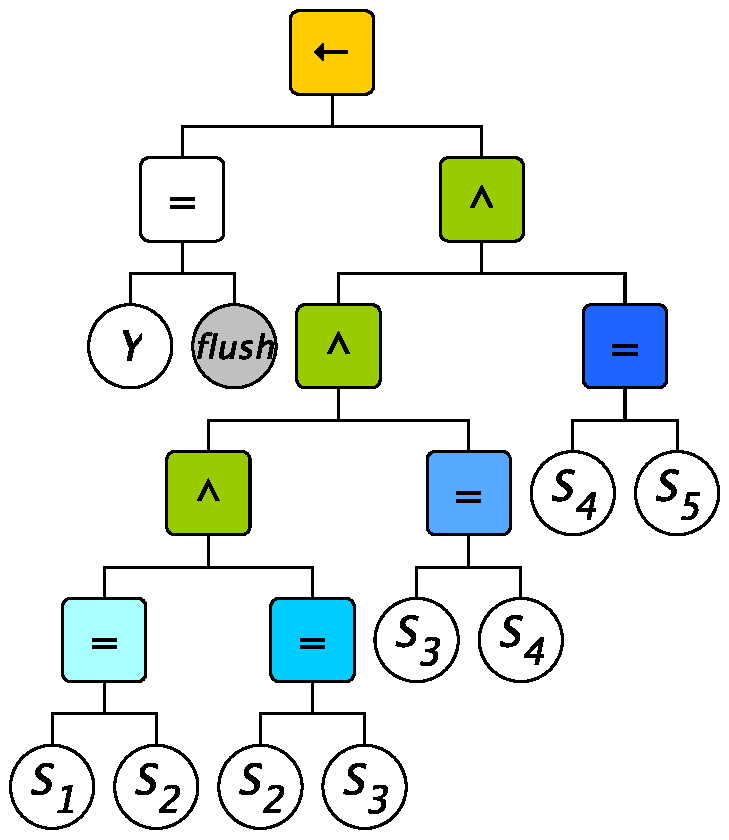
\includegraphics[width=\linewidth]{figures/ast-flush-1.pdf}
        \caption{AST of a formula}
        \label{fig:ast-kins-unencoded}
    \end{subfigure}
    \hfill$\rightarrow$\hfill
    \begin{subfigure}[]{0.32\linewidth}
        \centering
        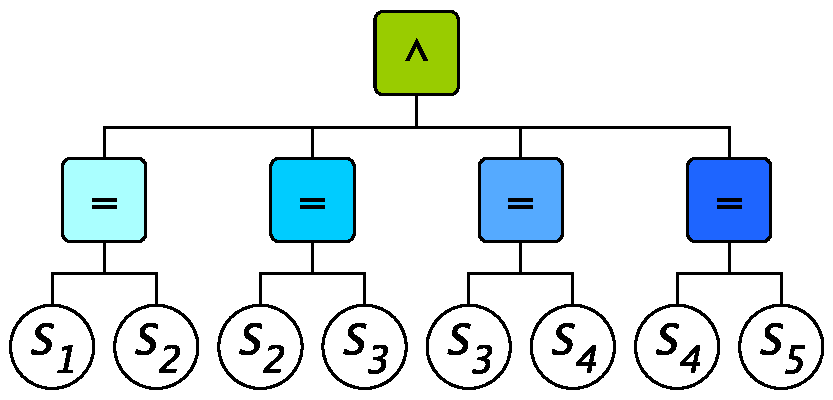
\includegraphics[width=\linewidth]{figures/ast-flush-2.pdf}
        \caption{Optimised AST of a formula}
        \label{fig:ast-kins-optimised}
    \end{subfigure}
    \hfill$\rightarrow$\hfill
    \begin{subfigure}[]{0.35\linewidth}
        \centering
        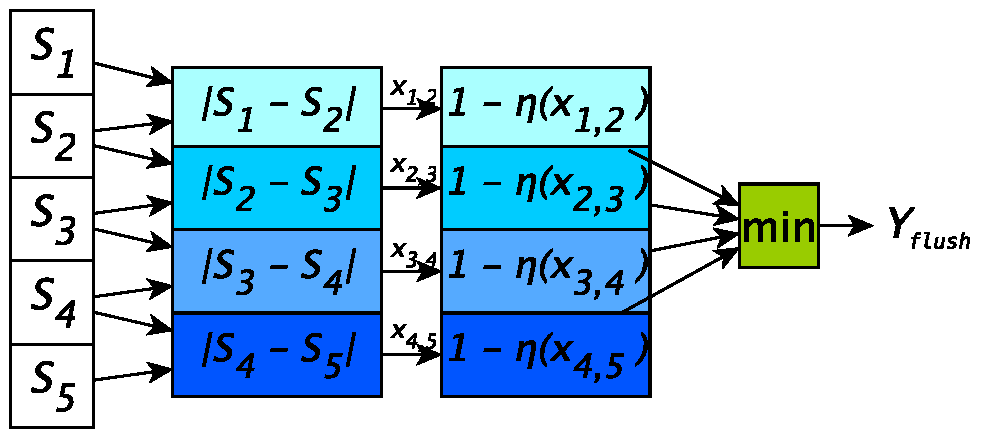
\includegraphics[width=\linewidth]{figures/net-flush.pdf}
        \caption{Layers from the optimised AST}
        \label{fig:net-kins-encoded}
    \end{subfigure}
    \caption[KINS Encoding of logic formulas into module networks]{
        %
        Example of the encoding process of formulas into module network.
        %
        Box coloured in the same way represent the encoding of a given operator through each encoding step.
    }
    \label{fig:ast-kins}
\end{figure*}

%
\begin{figure}
    \centering
    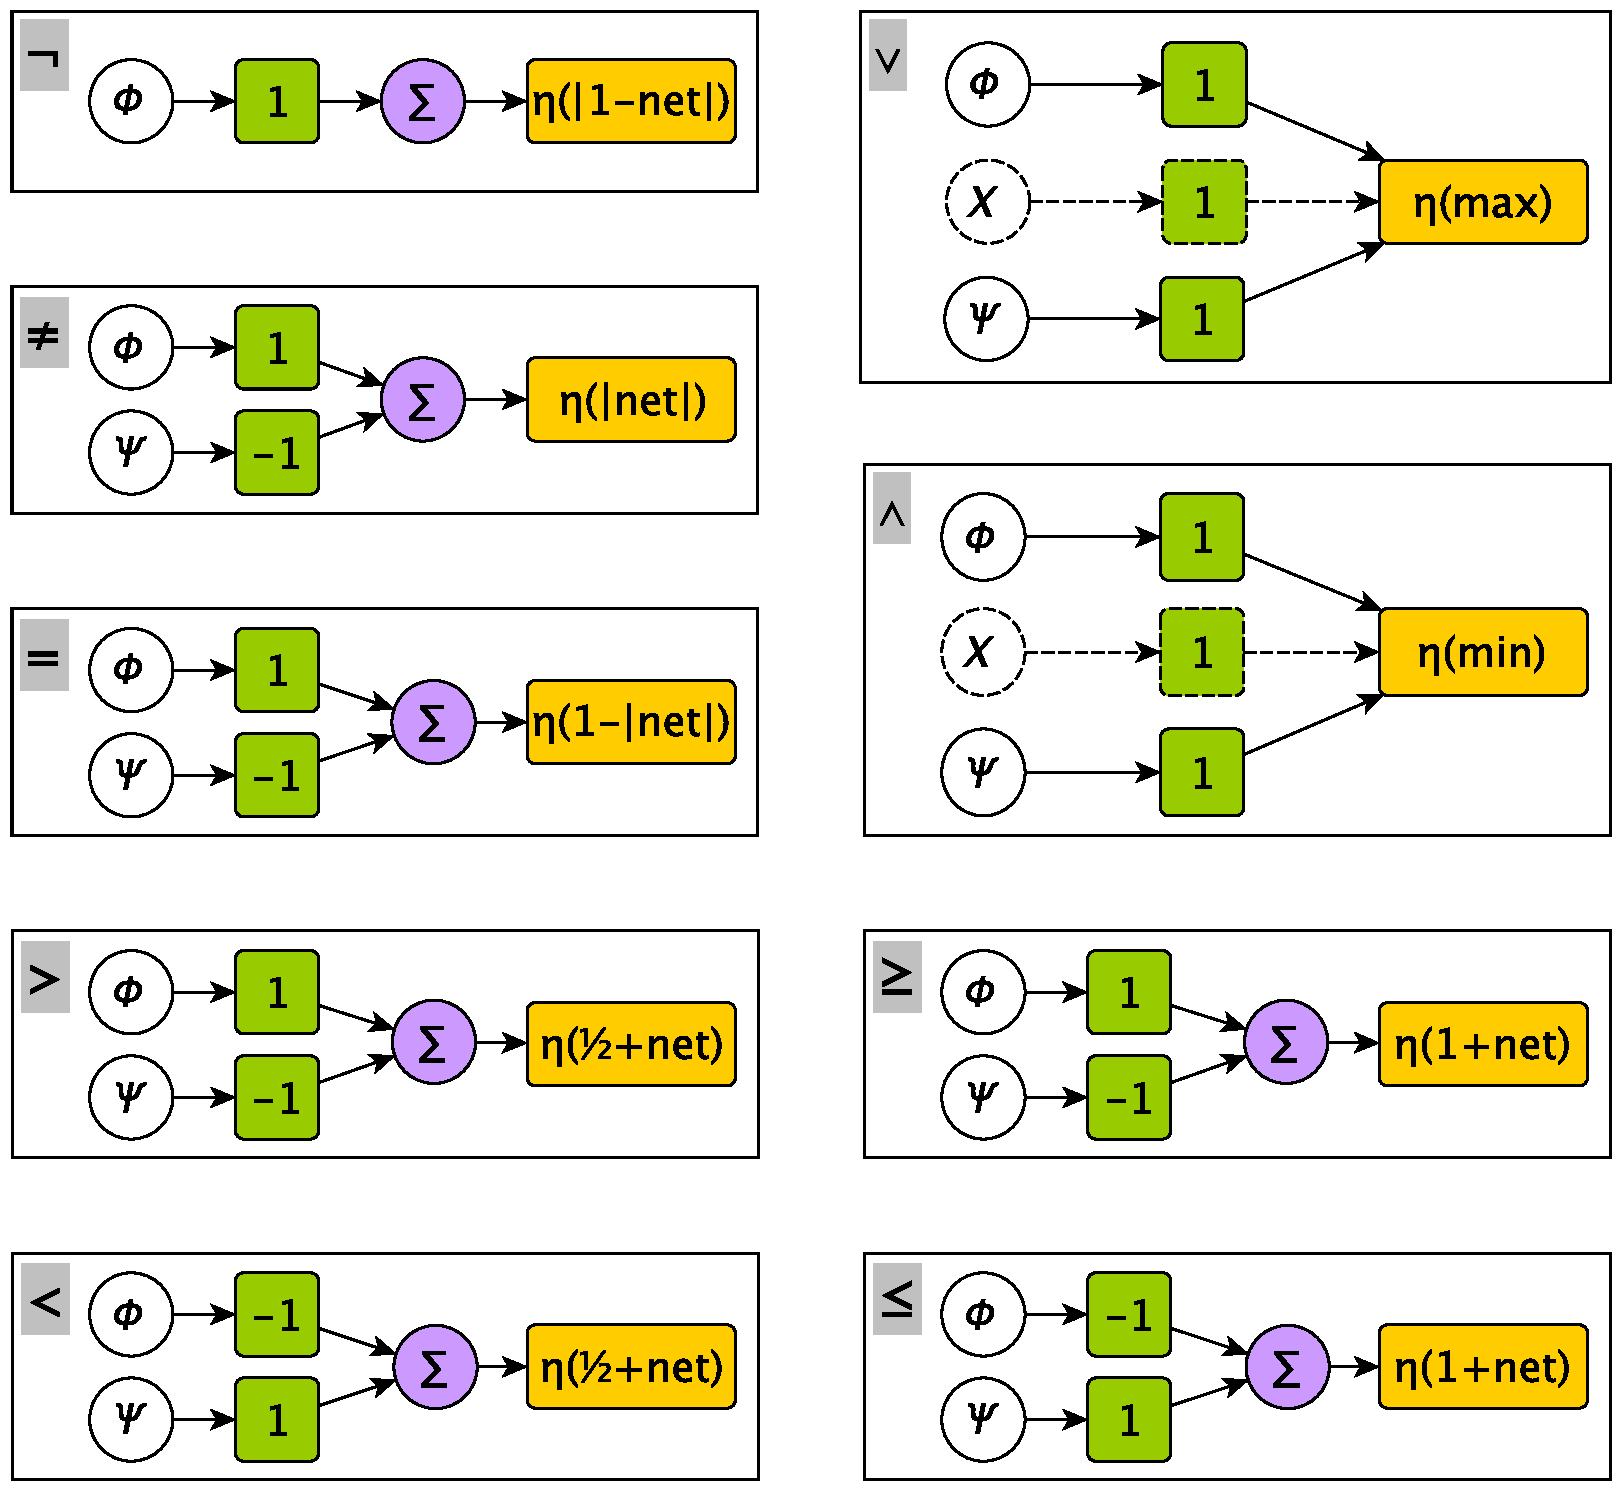
\includegraphics[width=0.8\linewidth]{figures/neurons}
    \caption[KINS mapping of formulas into neurons]{
        %
        \gls{KINS} mapping of formulas into neurons.
        %
        White circles are input variables ($I$), green boxes represent the corresponding weights ($W$), purple circles are the sum of the weighted inputs ($W x I$).
        %
        Yellow rectangles are activation functions, net is the output of $W x I$, maz and min respectively the maximum and minimum of input values, $\eta$ is the function described in \Cref{eq:eta-function}.
    }
    \label{fig:kins-neurons-mapping}
\end{figure}
%
By considering the same domain of the \gls{PHDS} used in \Cref{subsec:kill-validation}, we can take \Cref{eq:flush-class} as an example of a formula to be injected.
%
The procedure for encoding a logic formula into a dedicated neural module is illustrated in \Cref{fig:ast-kins}.
%
In this example, \Cref{eq:flush-class} is transformed into a neural module through three distinct phases.
%
First, the logic formula is parsed to construct its \gls{AST}, as shown in \Cref{fig:ast-kins-unencoded}.
%
Second, the \gls{AST} is simplified by merging commutative binary operators, as depicted in \Cref{fig:ast-kins-optimised}.
%
Third, the simplified \gls{AST} is encoded into a neural network, where each operator is mapped to a neuron that implements the corresponding operation, as specified in \Cref{tab:kins-logic-formulae}.
%
During the final step, the encoding rules defined in \Cref{fig:kins-neurons-mapping} are recursively applied to convert operators into neurons.
%
Input variables, such as \(S_i\), are represented as input neurons, while constants appearing in the formulas are mapped to neurons with fixed outputs.
%
Additionally, algebraic operations, including addition and multiplication, are implemented using single neurons that perform the respective operations.
%
This approach ensures that the symbolic knowledge is seamlessly integrated into the neural network structure.


\section{Discussion and future direction}\label{sec:ski-discussion-and-future-direction}